\documentclass[10pt, a4]{article}

\usepackage[T1]{fontenc}
\usepackage{cogsci}
\usepackage{pslatex}
\usepackage{gb4e}
\noautomath

\usepackage[round]{natbib}
\usepackage{graphicx}

\usepackage[english]{babel}

\usepackage{blindtext}

\graphicspath{{img/}}

\title{Do adults behave like children when under pressure?\\
\large Investigating adults' interpretation of universal quantifier under high cognitive load}

\author{{\large \bf Samuel Giacomelli (S.Giacomelli@student.rug.nl)} \\
University of Groningen}

\begin{document}

\maketitle

\begin{abstract}
    In the past a lot of researchers focused on children's atypical interpretation of different kind of quantifiers
    and they suggested that this behavior is caused by the underdeveloped cognitive resources that they have available
    when the task of interpreting a sentence containing quantifiers shows up. We start from their suggestion and in
    particular from the one given by \cite{minai2012hinders} with the intent to investigate wether this kind of atypical
    behavior can be owned also by adults that for some reasons are under pressure (i.e. have limited cognitive resources
    available). We propose a study that involves the completing of a Truth Value Judgment, along with a Digit Span, task,
    to try to prove that also adults can give an atypical interpretation to universal quantifiers. In this study we will
    record also the position of the cursor in order to be able to spot strange behaviors in the process of deciding the
    right answer to the proposed question.
\end{abstract}

\section{Introduction}
\subsection{Atypical universal quantification}
In the past year the tendency for children to give atypical interpretation to sentences containing universal quantifiers (e.g. \textit{each}),
has been studied deeply. In the first works they were just claimed to exhibit atypical universal quantification (\cite{piaget1964early}), and
later studies proved that children attribute to the extra objects, or extra subjects contained in the picture the cause of their atypical answer (\cite{philip1994event}).
In that study when children, from three to five years old, were presented a question like \textit{"Is every man wearing a hat?"} along with a picture showing
some men wearing a hat and an extra hat, they would answer \textit{"No"} pointing to the extra object (i.e. the hat) as the reason of their answer.
This kind of interpretation takes the name of \textit{SYMMETRICAL RESPONSE} (SR), because of the fact that the extra object ruins the situation
of symmetry depicted in the picture. On the other hand, adults' typical response is called \textit{LOGICAL READING} (LG), since adults' answer to the
former question would have been \textit{"Yes"} and it would have been the output of a logical analysis of the picture given the sentence.
A recent study by \cite{minai2012hinders} proved that children are capable of reaching both of the kind of responses and that what lets them give a
LG response is the level of cognitive development, which they tested through a Dimensional Change Card Sorting task.
The question that came on our mind after knowing about their results was \textit{"If children give SR responses do to their limited cognitive capabilities,
does it also work with adults that for some reason are under pressure or have they working memory particularly loaded?"}.

\subsection{Present Study}
Is exactly on this question that this study is based. This research will try to find out if there is a connection between
the limited size of the available working memory and the interpretation of the universal quantifier \textit{every}. To do this
we will base on the work of \cite{minai2012hinders}, gaining inspiration from the sentences they used and also, but just partially,
from the methodology of their study. We will make our participants, which will be both children (between 4 and 5 years old) and adults
(between 20 and 40 years old), perform a Truth Value
Judgment (TVJ) task (\cite{crain2000investigations}). The participant will be shown images representing a scene, like the one in Figure
\ref{img-target-sample}a and after some time they will hear a sentence and after that they will have to move the mouse toward the box
containing the "YES" answer, if they think that the image is representative of the sentence, or "NO" if they don't think so.
A mouse tracker software (\cite{freeman2010mousetracker}) will be used to record continuous data about the position of the cursor during
the process of decision making. This will let us know if there will be a difference in that process between the situation of \textit{LOW}
and \textit{HIGH} cognitive load. While our participants perform the \textit{TVJ} task they will be asked to perform also a Digit Span (DS)
task (\cite{conway2005working}) in order to gradually lower their available working memory and therefore their cognitive resources. This second task
will be presented in two different ways to children and adults taking in account that working memory is less developed for children.
Data collected from this two experiments will be not only the one from the right (i.e. LG) or wrong (i.e. SR) responses to the \textit{TVJ}
task, but also the one coming from the mouse tracking software, which will let us calculate the trajectories, the Medium Deviation, the Area
Under the Curve and the Reaction Times. We will analyse this data in order to find a bound between the decreasing number of available cognitive
resources and the increasing number of \textit{SR} response, but also to investigate wether the \textit{HIGH} cognitive load caused by the
\textit{DS} task will increase the duration of the process of deciding what is the right answer or will cause our participants to waver more.
This findings might lead the way to a lot of other researches on the linking between linguistic and cognitive skills, that might for example
be able to prove an increase in the time needed to process ambiguous sentences and might have useful applications in situations of emergency
where the indications should be as less ambiguous as possible in order to take little time as possible to be processed and understood.
In the following sections it's possible to find a more detailed explanation of all the different components of the experiment and also an anticipation
about how the data will be analyzed and which kind of result we expect.

\section{Method}
\subsection{Participants}
Our participants will be divided in two groups. The first one will be the \textit{CONTROL} and is going to be composed by around 40
english acquiring children between 4 and 5 years old, because in the study done by \cite{minai2012hinders}, they
proved that children in this age span are able to access both \textit{SR} and \textit{LG} responses, while the \textit{TARGET} group will consist
of at least 40 english native speakers adults between 20-40\footnote{Subjects in this age span should have completely developed
their linguistic and cognitive skills} years old. Both the \textit{CONTROL} and the \textit{TARGET} group will be composed in equal
parts by males and females in order to provide more consistent and reliable data for the analysis.
The participants of the CONTROL group will have to complete just the \textit{TVJ} task to determine the baseline of the childlike behavior,
while the one composing the TARGET group will have to complete both the \textit{DS} and the \textit{TVJ} task simultaneously.\\

\subsection{Procedure}
\subsubsection{TVJ}
Participants will be placed in front of a screen reporting in the beginning just a button with the label \textit{START}
in the centre-bottom of it. After having clicked on this button, a picture will be presented in the top centre of the
display followed after 2500ms by a spoken sentence. In the exact moment in which the subject starts hearing the sentence
he has to move the mouse toward the answer they think it is correct, in our case the possible answers are "YES/NO"
and are presented in two boxes on the left and on the right of the picture (at the exact same distance from the centre and the start button
to let us collect consistent information about the trajectories). If the subject is too slow in the beginning he/she will be asked to
start moving the mouse earlier. In order to display the following picture and so the following step of the task the subject has to click
on the start button (which will appear in the same position as before) again. Knowing that this kind of procedure might be demanding
for the children we take in account the possibility for them to take a break during the execution of the experiment (exactly in the middle of it, before
the beginning of the combined \textit{TVJ}-\textit{DS} task), while adults won't be able to take a break, because at that moment
they will be also in the middle of their \textit{DS} task.

\subsubsection{DS}
Both children and adults (i.e. \textit{CONTROL} and \textit{TARGET}) will be asked to go through a Digit Span (\textit{DS}) task
while performing the \textit{TVJ} one. This task consists in remembering a sequence of variable length, for children it will be of three numbers,
while for adults it will be made of six numbers, and, at the end of the \textit{TVJ} task, recalling the sequence in the exact order
in which it was presented. For both adults and children the single digits will be displayed on the screen for one second between the steps of the
\textit{TVJ} task, but there will be some difference in the presentation patterns between adults and children that we are going to explain below.

\subsubsection{Adults}
When adults press the start button for the first time a digit will appear on the screen and will stay there for 1 second. After this period of time the first part of the \textit{TVJ}
task will begin and after three steps this procedure will be repeated and another digit will be shown on the screen.
In this way, they will have to remember a total of six digits which in accord of the findings of \cite{taub1972comparison}
is a little bit below the maximum number of digits that an average 30yo adult can remember. The way chosen to propose the \textit{DS} task is specifically
thought to progressively increase the load on the working memory of the subjects, letting them with less available cognitive resources
to process the response to the \textit{TVJ} task's questions and trying to elicit in them a childlike behavior.

\subsubsection{Children}
The \textit{DS} task for children doesn't start with the first step of the \textit{TVJ} task, but after the break in the middle of it,
because children's working memory has a more limited capacity and they won't be able to remember the six numbers.
In this way, at the end of the experiment, they will have to remember just three digits.\\


\subsection{Materials}
\subsubsection{Sentences}
As this study is partially inspired by the work of \cite{minai2012hinders}, the stimuli used for the \textit{TVJ} task are the
english translations of the ones presented in their paper, with the only difference that is necessary to add a
\textit{filler item} in order to have an even number of stimuli, which are necessary to divide the task in two blocks.
The stimuli sentences are therefore 18 and are divided in three groups, respectively: 8 target sentences, 8 filler sentences
and 2 warm-up sentences. Below we report an example of a target sentence (\ref{sample_target_sentence}).
All the sentences will be spoken by both a male and a female english native speaker and
recorded in order to be presented to the participants in form of an audio track.

\begin{exe}
    \ex  Every turtle is holding an umbrella. \label{sample_target_sentence}
\end{exe}

Differently from \cite{minai2012hinders} we associated to the target sentences both the exhaustive and underexhaustive scenes. This means
that we have 2 different showable images for each sentence, which also require two different answers; in the case in which
the heard sentence is (\ref{sample_target_sentence}), the expected answer will be respectively "YES", when Figure. \ref{img-target-exhaustive} is showed,
and "NO", when Figure. \ref{img-target-underexhaustive} is showed. Past studies (\cite{drozil200112}) proved that children give wrong answers in both cases.
Participants are presented in the same proportion exhaustive and underexhaustive ones, respectively four for each type, but they are
never presented the same sentence with the two different images that depict it, in order to avoid priming.
In addition another change will be done on the images used in the above cited study that consist in moving the extra object in different positions
of the image. Since in the original paper they were always in the bottom right lattice, we think that this disposition made the children focus their
attention always on a minimal part of the image and in particular on the extra objects. Lastly, we kept just one of the two types of images
used in the above cited work, which is the Multiple Object one. We decided to keep this set of images because they, and more precisely with exactly
three extra objects, because they were proven to be able to elicit both \textit{SR} and \textit{LG} responses in children and therefore suggest to
do the same also with adults with a \textit{HIGH} cognitive load. Below (Figure \ref{img-target-sample}) we report an example of the images that
will be used in our research. 

\begin{figure} [!ht]
    \begin{minipage}{0.48\textwidth}
      a)
      \centering
      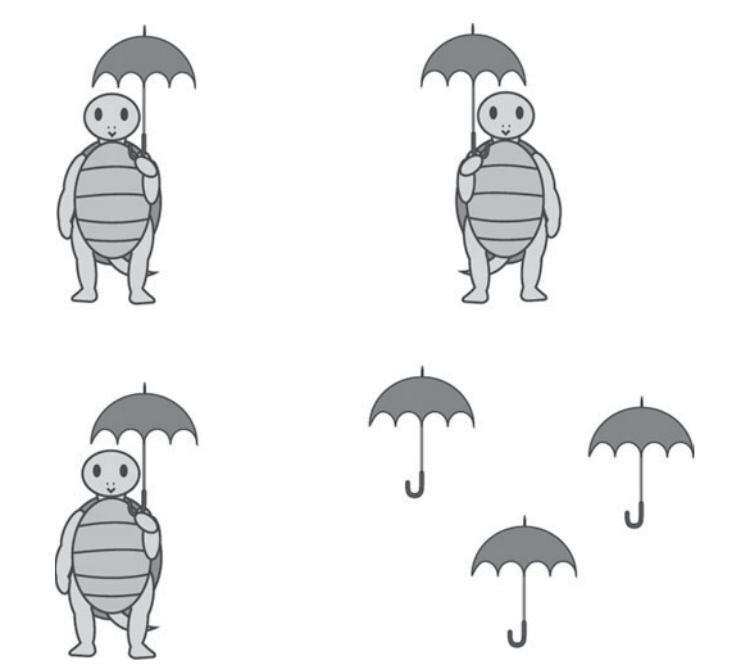
\includegraphics[width=.7\linewidth]{proj_prop_turtles_exhaustive.png}
      \label{img-target-exhaustive}    
    \end{minipage}
    \begin {minipage}{0.48\textwidth}
      b)
      \centering
      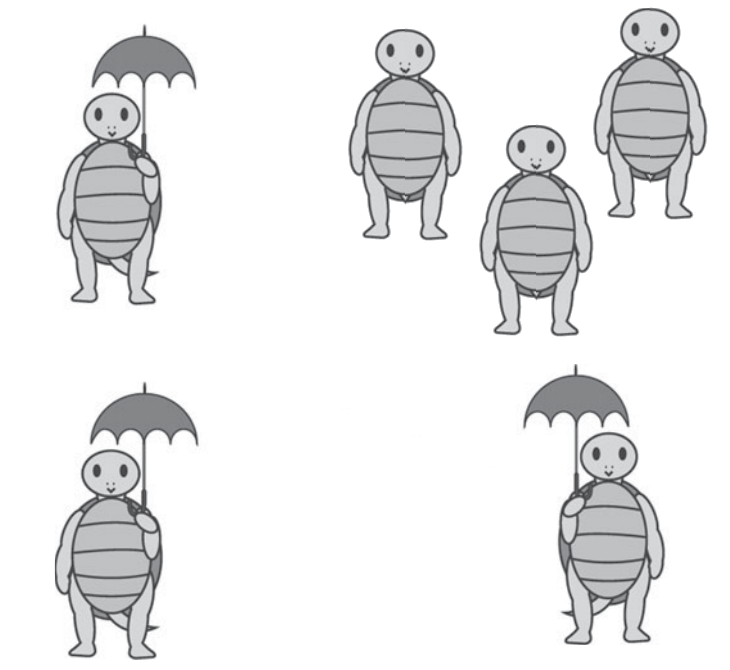
\includegraphics[width=.7\linewidth]{proj_prop_turtles_underexhaustive.png}
      \label{img-target-underexhaustive}
    \end{minipage}
    \caption{Example of images that will be used in the experiment. Picture a) shows the exhaustive case, while picture b) the underexhaustive one.}
    \label{img-target-sample}
\end{figure}


\subsection{Digits' sequences}
The stimulus sets consisted in sequences of six digits each (one every three steps of the \textit{TVJ} task), each of them from 1 to 9 without
repetition within the same sequence. Furthermore, according to the work of \cite{taub1972comparison} one more restriction will be applied on the sequences,
which consists in not presenting adjacent pairs of digits in the correct counting order (neither increasing or decreasing).\\

\section{Results}
\subsection{Data Analysis}
Since every subject will perform a \textit{TVJ} task and the technology used to design it concerns the use of the mouse tracker,
we will be able to collect not only the final answer of the subjects but also some information about the process of decision
making. We will analyse the percentage of \textit{SR} and \textit{LG} responses in children and adults to see wether
the adults behave in the same way that children do while performing both the \textit{TVJ} and the \textit{DS} tasks.
To analyse the data we will divide the one collected from both adults' and children's \textit{TVJ} task in two blocks, one containing 
the answers given in the first half of the task (when the working memory load was still low for adults and absent
for children), and the other one containing the answers given in the second half (with the maximum cognitive load for both of
the groups). In this way we will be able to see wether there is a relation between the increasing cognitive load and the tendency
to give childlike responses, but also if the responses given by children are influenced too by the higher cognitive load.
This approach will lead in an ANOVA analysis of the average \textit{LG} and accordingly \textit{SR} responses with a (2) group
x (2) cognitive-load design, where both group (\textit{CONTROL} vs \textit{TARGET}) and cognitive-load
(\textit{LOW} vs \textit{HIGH}) are between subjects factors.
Continuous data about the decision making process that starts with the presentation of the audio stimuli will be analyzed
in order to see wether there is: \textit{(a)} a commitment toward the wrong answer to the question (and so toward the
wrong interpretation of the scene) when the workload is \textit{HIGH} in adults, \textit{(b)} a similarity in the trajectories of the
decision making process of adults with a \textit{HIGH} working memory load and children with a \textit{LOW} one, \textit{(c)} a similarity in the values
relative to the Maximum Deviation (MD) from the ideal trajectory and the value of the Area Under the Curve (AUC) between
adults with a high working memory load and children and \textit{(d)} a increment in the Reaction Times in adults with a \textit{HIGH}
cognitive load meaning that they need more time to choose the right answer to the question.

\subsection{Expected Results}
The results that we expect from the above described analysis are multiple. First of all, when it comes to the analysis of the
average of \textit{LG} responses between the two groups and the two different levels of cognitive load, we expect to see a higher
percentage of \textit{SR} responses in both adults and children in a situation of \textit{HIGH} cognitive load. When looking at
the differences between the two groups we expect to notice that the percentages of \textit{LG} responses for children in a condition
of \textit{LOW} cognitive load is very similar to the one of adults with \textit{HIGH} cognitive load. If that's the case
we will be able to prove our initial hypothesis on the basis of the data acquired thanks to this experiment.
Second of all, when it comes to the analysis of the mouse tracker data, we expect to see a similarity in the trajectories
of children with a \textit{LOW} cognitive load and adults with a \textit{HIGH} one, depicting that the decision making process
of subjects belonging to the two different groups are very similar under this condition. Furthermore, we expect to see a commitment
toward the wrong answer when analyzing mouse tracking data about adults in a condition of \textit{HIGH} cognitive workload. Maybe
the cognitive load won't be enough to make them go for the wrong answer but if our hypothesis is true we will also be able to see that
adults are more on the fence and need further reasoning, so more time, to choose the right answer.\\

\section{Discussion}
In this study we investigated the role of the working memory in the interpretation of the universal quantifier \textit{every}.
We wanted to prove that with a limited cognitive capacity adults tend to behave like children (i.e. provide a \textit{SR})
when a sentence like (\ref{sample_target_sentence}) is presented combined to one of the two images in Figure \ref{img-target-sample}.
If our results will prove this childlike behavior it will mean that we found a cue that linguistic capabilities are strongly connected
and more interestingly strongly dependent on cognitive capabilities. It will also provided some support to the thought that
the linguistic development in children directly depends on their cognitive development. It will open the doors for lots of possible
researches about the relation between the two, for example one could try to answer the question \textit{"Are people slower in disambiguating
ambiguous sentences when they are in the situation of a high cognitive load?"}, but at the same time it may answer question proposed
from the opposite point of view, such as \textit{"Does the process of disambiguation of ambiguous sentences reduce our free working memory?
And how much?"}.

\bibliographystyle{plainnat}

\setlength{\bibhang}{.125in}
\setlength{\bibindent}{-\bibhang}

\vfill
\pagebreak

\bibliography{giacomelli_samuel_pp}

\end{document}
